% !TEX root = ./main.tex
\section{\gcoql}\label{sec:form}

In this section we describe our formalization of \gql in \coq. We start by defining a schema and its properties, then the graph data model and finally we review queries and their semantics. The definitions are as close as possible with respect to the \spec. This eyeball correspondence between the definitions in prose and the code gives a first level of trust that our formalization is correct.%, following the examples of X, Y and Z.
Whenever there is a mismatch we point it out and explain the reasoning behind each decision. 


\subsection{Schema}\label{subsec:schema}
We formalize schemas and type definitions following the \spec. A schema is represented as a record, containing a list of type definitions and a root type that specifies the available selections (\eg \texttt{Query} in the example from Figure \ref{fig:schema_ex}):
%

\begin{minted}[bgcolor=coqbg]{coq}
Record graphQLSchema := GraphQLSchema {
    query_type : Name;
    type_definitions : seq TypeDefinition }.
\end{minted}
%
Schemas may also include additional root types for specifying mutations and subscriptions (\cf\S3.2.1~\cite{gqlspec}). These operations are, however, out of the scope of our formalization.

Our formalization of type definitions closely follows the \spec, as
depicted in Figure~ \ref{fig:types_def}. A type may be a scalar type,
an object type, which possibly implements a set of interfaces, an
interface type, a union type or an enumeration type. Object and
interface type definitions comprise an (ordered) set of fields; union
types are defined by a set of type names and enumeration types by a
set of values. For the corresponding type definitions to be valid, all
such three sets should be non-empty. While the \spec enforces this
requirement syntactically (see the grammar on the left of Figure~\ref{fig:types_def}), we perform this validation when verifying the (overall) well-formedness schemas.     
%
\setlength{\grammarparsep}{10pt plus 1pt minus 1pt} % increase separation between rules
\begin{figure*}[h]
    \centering
    \begin{subfigure}{.5\textwidth}
    \begin{displaymath}
    \small
	\begin{array}{rl}
	\mathit{TypeDefinition} & ::= \\
	 | & \texttt{scalar } \name  \\
	 | & \texttt{type } \name\; (\texttt{implements } \name^{+})^{?} \texttt{ \{} \mathit{Field}^{+} \texttt{\}}\\
	 | & \texttt{interface } \name \texttt{ \{} \mathit{Field}^{+} \texttt{\}}\\
	 | & \texttt{union } \name \texttt{ = } \name\; (\texttt{|} \name)^{*}\\
	 | & \texttt{enum } \name \texttt{ \{} \name^{+} \texttt{\}} \\
	& \\
	\mathit{Field} & ::= \name \texttt{ (} \mathit{\overline{Arg}} \texttt{) : } \mathit{Type}\\
	& \\
    \mathit{Arg} & ::= \name \texttt{ : } \mathit{Type}\\
	& \\
    \mathit{Type} & ::=\\ 
     | & \name \\
 	 | &  \texttt{[}  \mathit{Type} \texttt{]}
	\end{array}
	\end{displaymath}
	
    
    %\fo{We may also want to use a less pompous grammar here}
    \end{subfigure}%
    \begin{subfigure}{.5\textwidth}
    \begin{minted}[bgcolor=coqbg]{coq}
    Inductive TypeDefinition : Type :=
    | ScalarTypeDefinition (name : Name)
    | ObjectTypeDefinition (name : Name)
                           (interfaces : seq Name)
                           (fields : seq FieldDefinition)
    | InterfaceTypeDefinition (name : Name)
                              (fields : seq FieldDefinition)
    | UnionTypeDefinition (name : Name)
                          (members : seq Name)
    | EnumTypeDefinition (name : Name)
                         (members : seq EnumValue).

    Inductive type : Type :=
    | NamedType : Name -> type
    | ListType : type -> type.
    \end{minted}

    \end{subfigure}
    \caption{Definition of \gql types: (left) \spec grammar; 
    (right) \gcoql definition.\newline
    {\footnotesize The $(\cdot)^{?}$ notation denotes optional attributes, and the overline $\overline{\cdot}$ denotes a sequence of elements.} 
    % \td{Changed the optional bracket here also -- to $( )^{?}$}
    % \td{Also changed $\overline{Field}$ bc the grammar specifies at least one}
    % \et{overbar or * -- you are using both. any difference?}
    % \td{No, just that I am not sure what to use}
    % \et{can a union have only one name? (ie. should it be + instead of *?)}
    % \td{Yep, it can have a single name (the thing is that each name is separated by a |)}
    }
    % \fo{In the grammar, I would push the scalar case to a new line, to match the \coq snippet on the right} \et{done}
    \label{fig:types_def}
\end{figure*}


% As can be seen from the figure, our implementation looses information about non-emptiness of fields, union and enum members. We push this validation to a posterior predicate, as well as the discussion about the reasons behind this decision, to the following paragraphs.

% As can be seen in the figure, we tried to match the \spec's definition as much as possible. This eyeball correspondence gives us a degree of confidence about the implementation.  % We currently do not include the \textit{Input Object} types, as well as anything related to \textit{introspection}.

In this regard, observe that the provided definitions of schema and types allow building ``invalid'' schemas. For instance, one can build an object that implements scalar types or use a nonexistent type as the query type. To avoid this problem, the \spec provides several validation rules, scattered throughout the document (though most can be found in \S3~\cite{gqlspec} under each type description).
 % the \textbf{Type Validation} subsection of each type described in ..  
 We gather all these rules and refer to them as the \textit{well-formedness}
condition of a \gql schema:\footnote{In \HP, this notion is called {\em consistency}.}

\begin{definition}
A \gql schema is \textit{well-formed} if: 
\begin{itemize}
    \item its root type (is defined and) is an object type, 
    \item there are no duplicated type names, and
    \item every type definition is \textit{well-formed}.
\end{itemize}
\end{definition}

In \gcoql, this is captured by the Boolean predicate below. %As mentioned in the introduction, our formalization heavily relies on Boolean reflection, following the SSReflect mindset.
%
\begin{minted}[bgcolor=coqbg]{coq}
Definition is_a_wf_schema (s : graphQLSchema) : bool :=
      is_object_type s s.(query_type) &&
      uniq s.(schema_names) &&
      all is_a_wf_type_def s.(type_definitions).
\end{minted}
%
% \et{naming inconsistency between is\_a\_wf\_schema and is\_wf\_typedef: skip the "a" in the case of schema}
% \td{I had actually renamed it is\_a\_wf\_typedef. I prefer with the "a" tbh}
The notion of well-formedness for type definitions requires \eg that
union members contain existent object types and that object and
interface types contain at least one field. Due to space limitations,
we omit the full definition and refer the interested reader to our
\coq development. %file \texttt{SchemaWellFormedness.v}.

%We will, though, resume the discussion about non-emptiness of fields, union and enum members, which are included in the predicate. The main reason behind this decision is that, even though the \spec embeds this information in the grammar, it still includes it in their validation rules later on. We believe that it is simpler to use common lists instead of defining new structures or using dependent types, from an implementation point of view, while still preserving the correspondence to the algorithmic description given by the \spec.
%\td{Not sure if correctly worded... but it was just simpler to use lists. A non-empty list structure required coercions to lists and then redefining some lemmas and things. Or using dependent types (sigma type) adds complexity when proving and defining things (at least that was the case for me)}


% There are two main reasons why we push this rule to a separate predicate instead of embedding it in the structure itself. The first one is that, even though the \spec embeds it in the grammar, it still includes it in a validation rule later on. To match their definition and preserve the eyeball correspondence, we also include it. The second reason is that we use SSReflect and it is simpler to use \mintinline{coq}{seq} directly and all its theory, instead of defining coercions and repeating definitions for a new structure.

For convenience, we encapsulate schemas with their well-formedness
proof in a single structure. 

%This structure also contains the
%predicate \mintinline{coq}{is_a_valid_value}, which determines whether
%a value used in a query or a node's property indeed matches the scalar type expected by the
% schema. For example, if a field argument has type \texttt{Float}, the
% \spec requires that the actual argument value represents a double-precision fractional number\footnote{The \spec declares a set of minimal scalar values and how they should be represented, such as floating-point values adhering to IEEE 754. We do not include this base restrictions but leave it open to implementation.}. To model values across our development, we parameterize each module with a type \texttt{Value} (of type \texttt{eqType}, \ie \mintinline{coq}{Variable (Value : eqType)}).
% An element in \texttt{Value} is either a scalar or a list of other values.
%

\begin{minted}[bgcolor=coqbg]{coq}
Record wfGraphQLSchema := WFGraphQLSchema {
    schema : graphQLSchema;
    _ : schema.(is_a_wf_schema); }.
\end{minted}

%\fo{Mention what \texttt{Vals} represents (used here for the first
%  time, but not defined)}


% This predicate is necessary to establish when a value used in a query or in the graph actually matches the scalar type expected by the schema. For instance, if an argument requires a \texttt{Float} value, then the actual value passed to the query must be something that represents a double-precision fractional value\footnote{The \spec declares a set of minimal scalar values and how they should be represented, such as floating-point values adhering to IEEE 754. We do not include this base restrictions but leave it open to implementation.}. This predicate validates that this is satisfied.

% Due to space constraints, we omit the definition of \textit{well-formedness} for type definitions. This property includes things such as: interfaces and objects must declare at least one field, objects correctly implement their declared interfaces, union types are not empty and contain only object types, amongst others. These definitions are collected from the \spec \td{Scattered throughout the \spec*}.

Having reviewed our formalization of schemas, we now discuss our formalization of the data model. 



\subsection{Data Model}\label{subsec:graph}
Following \HP, we adopt a data model based on graphs, where data are
modeled as directed property graph, with labeled edges and typed
nodes. Nodes contain a type and a set of properties (key-value pairs)
and  edges contain single labels that describe the relations between
adjacent nodes. Also, every property and label may contain a list of
arguments (key-value pairs). %Refer to Figure~\ref{fig:graph_ex} for an example.

%To represent the values associated to properties and arguments, we consider the type \Vals. 
% A value in \Vals may be a single scalar value or a list of values\td{This choice is based on the limitations of the model}.\fo{I think we should address this in the Discussion section, where we discuss the limitations of our formalization. We could even remove the last sentence from the paragraph.}

\begin{definition}
A \emph{\gql graph} is defined by:
\begin{itemize}
    \item a root node, and
    \item a collection of edges of the form ($u$, $\fld$, $v$), where $u, v$ are nodes and
      $\fld$ is a label with arguments
      (key-value pairs).
\end{itemize}
\end{definition}

To model the values in a graph, as well as across the rest of our development, we define an inductive type \texttt{Value}, representing 
either scalar or lists of values. The corresponding modules are then parameterized by the
\texttt{Scalar} type.
\begin{minted}[bgcolor=coqbg]{coq}
Variable (Scalar : eqType).
Inductive Value : Type :=
| SValue : Scalar -> Value 
| LValue : seq Value -> Value.
\end{minted}

The definition of a graph in \gcoql is then captured by the following structures.
% A \texttt{label} represents the set of labels over an edge or keys in a node's property. 
%\td{Probably the name is not the best}\fo{Fully agree. I suggest changing \texttt{fld} to \texttt{label}, \texttt{Field} to \texttt{Label} and \texttt{label} to \texttt{name} (or \texttt{lname} if there is a clash) }. 
%
\td{The code actually looks like that, with the @ in every Value occurrence. Should we leave it or remove it for presentation?}\et{in practice, you could make it an implicit parameter instead of a variable, right? \texttt{Inductive Value \{Scalar : eqType\} : Type := ...}}
\et{in any case, in the paper, just use Value and forget about the Scalar argument}
\begin{minted}[bgcolor=coqbg]{coq}
Record label := 
  Label { lname : string; args : seq (string * @Value Scalar) }.

Record node := 
  Node { ntype : Name; nprops : seq (label * Value) }.

Record graphQLGraph := 
  GraphQLGraph { root : node; 
                 edges : seq (node * label * node) }.
\end{minted}
The root node of a \gql graph represents the starting point from where queries are evaluated. Note that edges are modeled as a list, and not as a set; unicity of its members is handled by a separate validation. 
 % and include a posterior separate validation on uniqueness of its members.
We found this approach to be more convenient in the current development, but this design decision would be fairly easy to revisit if needed.
% \td{Added this}


Intuitively, the data modeled by a \gql graph is expected to respect
(the type system described by) a schema. However, the definition of
graphs above is fully independent of schemas. To relate the data to the type system, we define the notion of \textit{conformance} of a graph \wrt a schema, partially based on~\cite{gqlph}.
%\td{Over here we should start including the notion of Value type + valid scalar}
%
\begin{definition}
A \gql graph $\mathcal{G}$ \textit{conforms} to a schema $\mathcal{S}$ if: \td{Should this definition include the predicate? \eg, with a value validation predicate bleble}\et{instead say that the value validation predicate is a global (module) parameter -- ok, seems you're doing that in the next paragraph below}
\begin{itemize}
    \item the types of $\mathcal{G}$ root node and $\mathcal{S}$ query
      root coincide,
    \item every node of $\mathcal{G}$ \textit{conforms} to
      $\mathcal{S}$, and
    \item every edge of $\mathcal{G}$ \textit{conforms} to
      $\mathcal{S}$. 
   
\end{itemize}
\end{definition}
%


The conformance of nodes validates that a node's type is declared as an object type
in the schema and that its properties are correct. In turn, a property is correct if 
its key and arguments are defined in a field in the corresponding type, and any value, either in an argument or
the property's value, is \emph{valid} \wrt the expected types described in the schema. 
For instance, if a field has type \texttt{Float}, 
then a node's property matching the field must have a value that represents a double-precision fractional value\footnote{The \spec declares a set of minimal scalar values and how they should be represented, such as floating-point values adhering to IEEE 754. We do not include these base restrictions but leave it open to implementation.}.
To model value validation throughout our development, we parameterize the corresponding modules with a predicate $ is\_valid\_scalar\_value : graphQLSchema \to Name \to Scalar \to Bool$.
\td{I am trying to push this definition here and then not having to redefine it or explain it again}\et{yep, that's better}
\td{Probably not the best name for the predicate tbh}
\et{what about check\_scalar ?}

Meanwhile, the conformance of edges validates that: (1) an edge's label corresponds to a field in the
source node's type, (2) the target node's type corresponds to the field's type (either the same type, an implementation
or part of a union), (3) if the type is not a list type then there should only be one outgoing edge, from the source node, with the given label,
and (4), the arguments are defined in the corresponding field in the schema and their values are valid \wrt their expected types.

%includes rules such as checking that a node
%type is declared as an object type in the schema and that its
%properties are defined as fields in the corresponding type. Among
%others, the conformance of edges ensures that edge labels are declared
%as a field in the source node's type and the target node has a type
%compatible with the field's return type. Full definitions of both
%these notions can be found in the \coq development. %are found in file \texttt{GraphConformance.v}.

With this in mind, the notion of conformance of a graph \wrt a schema is formalized as follows:
%
\begin{minted}[bgcolor=coqbg]{coq}
Variable (is_a_valid_scalar_value : 
  graphQLSchema -> Name -> Scalar -> bool).
  
Definition is_a_conforming_graph 
      (s : wfGraphQLSchema) 
      (g : graphQLGraph) : bool :=
  root_type_conforms s g.(root) &&
  edges_conform s g &&
  nodes_conform s g.(nodes).
\end{minted}
%
% As a side note, this notion was only loosely defined in \HP, but it is properly addressed in a recent work of one of its authors ~\cite{olafschema}.

Similarly to \gql schemas, we define a structure that encapsulates the notion of a \textit{conformed} graph, containing a graph and a proof of its conformance to a particular schema.
\td{Since I mention above that it uses this predicate and show it as a variable, maybe we can skip it?} \et{yes}
\begin{minted}[bgcolor=coqbg]{coq}
Record conformedGraph (s : wfGraphQLSchema) 
(*  (is_a_valid_scalar_value : graphQLSchema -> Name -> 
    Scalar -> bool) := *)
  ConformedGraph { graph : graphQLGraph;
                       _ : is_a_conforming_graph s graph }.
\end{minted}

 %These properties include validation rules such as: every node must have an object type and their properties must be defined in their associated type, or an edge's label must be declared as a field in the source node's type and the target node must have a type compatible to the field's return type, among other things.

%With both the schema and the underlying data model we can proceed to define \gql queries and their semantics.


\subsection{Queries}\label{subsec:query}
To define queries we faithfully follow the \spec, as shown in
Figure~\ref{fig:query_def}. A query consists of a list of selections, and can optionally be named.
% consists of an optional name
% \fo{We should mention this also in \S 2}\td{Not really necessary, or is it?} and a list of selections. 
A selection $\sel$ can be a single field $\fld$ with arguments, an aliased field $\afld$, or a possibly-aliased field followed by a set of subselections $\sset$, or an inline fragment $\ifrag{t}{\sset}$ comprising a type condition \texttt{t} and a set of subselections $\sset$. 
Whenever a field selection contains an empty list of arguments, we simply omit the \texttt{[$\args$]} and, instead, only use the field's name.

% Fields can be accompanied by a list of arguments and can also be renamed.

\begin{figure*}[h]
  \centering
  \begin{subfigure}{.5\textwidth}
  \begin{displaymath}
	\begin{array}{rcl}
	\query & ::= & \texttt{query } (\name)^{?} \texttt{ \{}  \sset \texttt{\}} \\
	&& \\
	\sel & ::= & \fld \\
	& | & \afld \\		
	& | & \nfld{\sset} \\
	& | & \anfld{\sset} \\
	& | & \ifrag{t}{\sset} \\
	\end{array}
	\end{displaymath}
	
	\iffalse
    \begin{grammar}
    		<Query> ::= [\textbf{\texttt{query}} [<name>]] \textbf{\texttt{\{}} <Selection>$^{+}$ \textbf{\texttt{\}}}
		
        <Selection> ::= <name> \textbf{\texttt{(}} <Arg>* \textbf{\texttt{)}}
        \alt <alias> \textbf{\texttt{:}} <name> [\textbf{\texttt{(}} <Arg>$^{+}$ \textbf{\texttt{)}}]
        \alt <name> [\textbf{\texttt{(}} <Arg>$^{+}$ \textbf{\texttt{)}}] \textbf{\texttt{\{}} <Selection>$^{+}$ \textbf{\texttt{\}}}
        \alt <alias> \textbf{\texttt{:}} <name> [\textbf{\texttt{(}} <Arg>$^{+}$ \textbf{\texttt{)}}] \textbf{\texttt{\{}} <Selection>$^{+}$ \textbf{\texttt{\}}}
        \alt \textbf{\texttt{... on}} <name> \textbf{\texttt{\{}} <Selection>$^{+}$ \textbf{\texttt{\}}}
        
        <Arg> ::= <name> \textbf{\texttt{:}} <value>
    \end{grammar}
    \fi 
    
  \end{subfigure}%
  \begin{subfigure}{.5\textwidth}

    \begin{minted}[bgcolor=coqbg]{coq}
    
    Record query := 
         Query { qname : option string; 
                 selection_set : seq Selection }.
                   
    Inductive Selection : Type :=
    | SingleField (name : Name)
                  (arguments : seq (Name * Value))
    | SingleAliasedField (alias : Name)
                         (name : Name)
                         (arguments : seq (Name * Value))
    | NestedField (name : Name)
                  (arguments : seq (Name * Value))
                  (subselections : seq Selection)
    | NestedAliasedField (alias : Name)
                         (name : Name)
                         (arguments : seq (Name * Value))
                         (subselections : seq Selection)
    | InlineFragment (type_condition : Name)
                     (subselections : seq Selection).
    \end{minted}
  \end{subfigure}
  \caption{Definition of \gql queries:
  (left) \spec grammar; 
  (right) \gcoql definition. %\et{why Vals instead of Val?}\td{This was to keep close similarity to \HP (way at the beginning) -- do you think Val is better?}
  \newline{\footnotesize Symbols \texttt{f}, \texttt{a} and \texttt{t} correspond to identifiers for field names, field aliases and type conditions, respectively.
  Symbol $\alpha$ stands for a key-value pair.}}
  % , representing the arguments of fields. \et{rather alpha is a key-value pair, and overbar is the list notation}}
  %\td{Brackets in optional query name may conflict with the others? It is a diff font, but idk if maybe using something else=}
  %\et{yeah that's a bit unfortunate. A solution is to use $( ... )^?$ to denote optional elements (without parenthesis when it's a single element)}
  %\td{Is it me or the query record looks flattened?} \et{???}
  %\td{To be completely accurate, the parenthesis in field selections are not necessary unless there are arguments}\td{This might add some noise?}\et{yeah I think that'd be too much (and not very relevant)}
  \label{fig:query_def}
\end{figure*}

Intuitively, a valid query and its selection set form a tree, where leaves correspond to fields of scalar types and inner nodes correspond either to fields of some object type or abstract type (\ie~interface or union),
% \fo{abstract type not defined}\td{Ok like this?} 
or to inline fragments that condition when their subselections are evaluated. 

\iffalse
%For instance, the query in Figure \ref{fig:qres_ex} can be depicted as the tree in Figure \ref{fig:query_tree}.
\begin{figure}
    \centering
    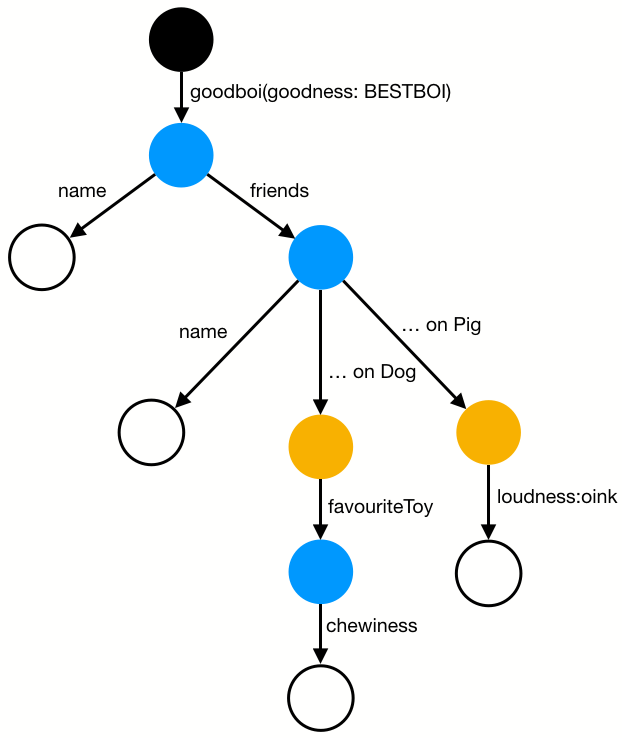
\includegraphics[scale=0.33]{imgs/query_tree.png}
    \caption{\gql query as a tree.}
    \label{fig:query_tree}
\end{figure}
\fi 

% Similar to the schema definition, we follow the \spec's grammar as closely as possible, as can be seen from Figure~\ref{fig:query_def}. We do not embed the property of non-emptiness of subqueries in the definition because the \spec pushes it to a different validation rule, even though it is already embedded in the grammar, and we believe it is simpler to reuse the \texttt{seq} library and its existent functionalities. 

Observe that the definition of queries in Figure~\ref{fig:query_def}
is not bound to any schema, requiring thus a separate validation
process to ensure that they adhere to a given schema. We introduce the
notion of query \textit{conformance}, based on a set of validation
rules scattered throughout the \spec (\cf\S5~\cite{gqlspec}). The
validity of queries depends on the validity of their selection sets,
which in turn requires the notion of \textit{type in scope} at a
given selection location\footnote{The \spec refers to it as the \emph{type in scope} or \emph{parent type}. Some algorithmic descriptions make use of the types in scope but are not explicit in their signatures.}. % Since queries are selections over the fields of types, it is important to know exactly to what type they are being applied.
To illustrate this, consider the following query with two occurrences of field \texttt{name}.

%\begin{minipage}[t]{.25\textwidth}
\begin{minted}[escapeinside=||, mathescape=true]{js}
query {
  goodboi {
    |$\ldots$| on Dog {
      name
      favoriteToy
    }
    |$\ldots$| on Pig {
      name
      favoriteToy
    } } }
\end{minted}
%\end{minipage}%
% \begin{minipage}[t]{.25\textwidth}
% \begin{minted}[escapeinside=||, mathescape=true]{js}   
% type Human {
%   age: Int
% }

% type Martian {
%   age: Float
% }
% \end{minted}
% \end{minipage}
%\et{for space reason, we may want to take some liberties wrt the formatting of queries and responses (see some examples on this page)}


\noindent In the first occurrence, the field is requesting information about the
\texttt{Dog} type, while in the second it is requesting information about the \texttt{Pig} type. The distinction is important because some field selections might be valid in some contexts but not in others. This is the case, for instance, for field \texttt{favoriteToy}: It is valid in the context of a \texttt{Dog} type but it is invalid in the context of a \texttt{Pig} type, as \texttt{Pig} type does not contain any such field. %Similarly, the above query would also be invalid if \texttt{Pig} type contained a so-called field, but of type different from \texttt{Toy} ---the type of the same field in type \texttt{Dog}.

%Just as in the case of well-formedness of schemas or conformance of graphs, queries must go through a validation process. We define the property of \textit{conformance} of queries, based on validation rules scattered throughout the \textit{Validation} section of the \spec\footnote{https://graphql.github.io/graphql-spec/June2018/\#sec-Validation}.

% Before describing the validation process, it is very important to address the notion of \textit{type in scope} where queries are defined and used. The type in scope is the type over which a user might be requesting information on its fields. To illustrate this, consider the following query. The first selection, namely \texttt{goodboi}, is requesting information about the query type, meaning that it is used in the context of the \texttt{Query} type. Moving onto the  \texttt{name} subselection, it is not direct which is. In one case, the type in scope is \texttt{Dog}, while in the other the field is used in the context of the \texttt{Pig} type.

% The importance of this type in scope is that fields or inline fragments might be valid in certain cases but not in others. Similarly, a field may have a particular return type in one case and a different one in another type, like in the following example. Both types have an \texttt{age} field, but in one case it returns an integer value while in the other a floating point value. If that field is encountered in a query, it is necessary to know to which type it is being requested.

Now that we have clarified the notion of type in scope, we are in
condition of defining the notion of query conformance, which in turn
depends on the notion of selection set conformance.

%\td{A query conforms when its selections conform to the Query type}
\begin{definition}
A \gql selection set $\sset$ \textit{conforms} to a schema $\schema$ over a type in scope $\mathit{ts}$ if:
\begin{itemize}
\item every selection in $\sset$ is  well-formed, and

\item any two field selections in $\sset$ are type-compatible and
  renaming-consistent\footnote{In the \spec
    (\cf\S5.3.2~\cite{gqlspec}), these two notions roughly correspond
    to \emph{having-the-same-response-shape} and
    \emph{fields-can-merge}, respectively.}.
       
\end{itemize}
\end{definition}

The first rule ensures that every selection is well-formed on its own, with
respect to the type in scope. Its requirements vary according to the
kind of selection. For instance, if the selection is a field, the rule
checks that the field is part of the type in scope and that its
arguments are correctly provided; if the selection is an inline
fragment, then the type condition must at least share one subtype with
the type in scope. This rule also includes validating the values used
in arguments, similarly to the case of graphs.


In the second rule, the type-compatibility requirement forbids the
selection set in \eg the following query:

\begin{minipage}[t]{.22\textwidth}
\begin{minted}[escapeinside=||,mathescape=true]{js}
query {
  goodboi {
    friends {
      |$\ldots$| on Dog {
        name
     }
     |$\ldots$| on Pig {
       name:oink
} } } }
\end{minted}
\end{minipage}%
\begin{minipage}[t]{.22\textwidth}
\begin{minted}[escapeinside=||,mathescape=true]{js}
// Possible invalid output
{
  "goodboi" : {
       "friends" : [
         { "name" : "Marle" },
         { "name" : 9000 }
     ]
} }
\end{minted}
\end{minipage}

Intuitively, the previous query is invalid because its evaluation can produce results with the same key 
(key \texttt{name}) but associated to values of different type (\eg string and integer values).

%\td{We are not exactly capturing that the fields can be inside fragments, is it ok?}\et{I don't get it}
The definition of field \emph{type-compatibility} is recursive. Two nested
field selections are type-compatible if whenever
they have the same response name, any two fields in the concatenation of their
subselections are also type-compatible. Two single field selections
are always type-compatible, unless they have the same response
name and different (scalar or enum) type.

Finally, the renaming-consistency condition ensures that fields with
the same response name refer to the same piece of information. For
instance:
% \td{This leaves a lot of empty space :/}
\begin{minted}[escapeinside=||,mathescape=true]{js}
query { goodboi {
          age   
          |$\ldots$| on Pig { age:oink } }
\end{minted}

Intuitively, this query is considered invalid because the fields with response name \texttt{age} both refer to distinct pieces of information;
the first occurrence refers to the age of the animal, while the second accesses the field \texttt{oink} but renames it accordingly.

%\fo{Add example and briefly explain} 

Two field selections are \emph{renaming-consistent} if whenever they have the
same response name and lie under overlapping types in context
\fo{@Eric, is there any standard terminology for this
  ``overlapping'', meaning that they share at least one subtype?},
  \et{sharing a subtype means that their "(subtyping) meet/glb" exists--is that what you're referring to?}
  \td{Yeah, at least I believe it is}
they have the same (actual) name, the same arguments and any two
fields in the concatenation of their subselections are also
renaming-consistent.

The last two rules are defined as a single validation rule in the \spec (\cf\S5.3.2~\cite{gqlspec}). 
We choose to split them because we noticed that they indeed can be defined separately, simplifying their implementation as well as facilitating 
reasoning about them\footnote{Our algorithm implements an optimized version of the rule. A team at XING recently published another optimized algorithm~\cite{xingalg}.}.


\begin{definition}
A \gql query $\query$ \textit{conforms} to a schema $\schema$ if its selection set conforms to $\schema$ over the query root type.
\end{definition}

%\et{this is the beginning of the problem I'm having with your statements about queries. There is the notion of *a query*, noted $\varphi$, yet from now on your statements are about *queries*. The definition below mixes "the content" (consistency, compatible response, etc.) with "the sequence" (all, list comprehension, etc). Worse, later on in the development, you use $\varphi$ as the variable name of type "seq Queries" (while fig6 uses a bar over). See also my later comments about your "plural formulations"}

\noindent In \gcoql, this is captured with the following predicates.
%\td{Updated}
%\td{Need to adjust names}
%The implementation can be seen in the code below, however due to space limitations we only informally describe the %three mentioned rules. The complete definitions can be found in the file \texttt{QueryConformance.v}.
\td{Similar case}
\begin{minted}[bgcolor=coqbg, escapeinside=@@, mathescape=true]{coq}
Definition query_conforms 
  (s : wfGraphQLSchema) (@$\query$@ : query)
(*  (is_a_valid_scalar_value : graphQLSchema -> Name -> 
    Scalar -> bool) *) : bool :=
    selections_conform s s.(query_type) @$\query$@.(selection_set).
    
Definition selections_conform (s : wfGraphQLSchema)
(*  (is_a_valid_scalar_value : graphQLSchema -> Name -> 
        Scalar -> bool) *)
  (ts : Name) (@$\sel$@s : seq Selection) : bool :=
    let @$\sel$@s_with_scope := [seq (ts, @$\sel$@) | @$\sel$@ <- @$\sel$@s] in 
      all (is_consistent ts) @$\sel$@s &&
      @$\sel$@s_with_scope.(are_type_compatible) &&
      @$\sel$@s_with_scope.(are_renaming_consistent).
\end{minted}

% This concludes the definition of \gql queries, the validation process and the notion of size of selections. 
From now on, it is assumed that queries conform to a given schema. Finally, most of the recursive definitions over selection sets are well-founded using a notion of size.
\begin{definition}[\cite{gqlph}]
% \td{It is in essence the same, except that they define selections along with queries}
The \emph{size} of a selection $\sel$ and selection set $\sset$, noted $\ssize{\cdot}$, is recursively defined as:
\begin{small}
\begin{align*}
    \ssize{\fld}  = \ssize{\afld} &=  1\\
    \ssize{\nfld{\sset}} = \ssize{\anfld{\sset}} = \ssize{\ifrag{t}{\sset}} &= 1 + \ssize{\sset}\\
    \ssize{\sset} &= \sum_{\sel_{i} \in\; \sset}{\ssize{\sel_{i}}}
    \end{align*}
\end{small}
\end{definition} 

%\td{Cannot define $\sset$ in Coq (lexer error), so I had to go with $\sel$ instead of the selection set and simply \texttt{sel} for an atomic selection}
 %\et{you can use "$\sel$s"}
%\fo{This introduces the conformance of a query \wrt a schema, but the schema is never mentioned in the definition. It needs to be fixed!!!}


%has to be valid with respect to the type in scope \fo{when can it not be valid?}\td{If both the type condition and the type in scope do not share at least one subtype (subtype is reflexive). Not sure if this is relevant here though}.%The \spec defines this rule in several different sections.

% The second rule validates when fields can be correctly merged during evaluation, which is an essential aspect of the semantics, since it ensures that repeated fields are only evaluated once. To illustrate this, consider the following query, where a user requests information on the fields \texttt{name} and \texttt{oink} of pigs. The user decides to rename the field \texttt{oink} to \texttt{name}, however this is invalid, since both fields cannot be merged and evaluated once; both fields refer to distinct pieces of information in the system.

% \begin{minted}[escapeinside=||,mathescape=true]{js}
% query {
%   goodboi {
%     name    
%     |$\ldots$| on Pig {
%       name
%       toy:oink
%     }
%     |$\ldots$| on Dog {
%       name
%       toy:age
%       }
% } } }
% \end{minted}

% The last rule is necessary to check when fields generate consistent values when evaluated. For instance, in the query below a user might request the names of dogs and the oinkness of pigs, but renaming the latter to have the same response name as the former. This query is considered invalid because evaluating it might produce a response that contains entries where the key \texttt{name} is associated to both string values and floating point numbers. 

% \begin{minipage}[t]{.22\textwidth}
% \begin{minted}[escapeinside=||,mathescape=true]{js}
% query {
%   goodboi {
%     friends {
%       |$\ldots$| on Dog {
%         name
%       }
%       |$\ldots$| on Pig {
%         name:oink
% } } } }
% \end{minted}
% \end{minipage}%
% \begin{minipage}[t]{.22\textwidth}
% \begin{minted}[escapeinside=||,mathescape=true]{js}
% // Possible invalid output
% {
%   "goodboi" : {
%     "friends" : [
%         { "name" : "Marle" },
%         { "name" : 9000 }
%     ]
% } }
% \end{minted}
% \end{minipage}




% The main issue is that the \spec allows for what we call \textit{invalid fragments}, originally described in an issue in the \spec's repository\footnote{https://github.com/graphql/graphql-spec/issues/367}. In a nutshell, the \spec allows using fragments with type conditions that can span to multiple unrelated types. These end up not being evaluated due to posterior checks\footnote{https://graphql.github.io/graphql-spec/June2018/\#DoesFragmentTypeApply()}.


% \td{This looks a bit weird... Should it be a "definition" or just inline it as \HP does?}





\subsection{Semantics}\label{subsec:semantics}
Now we have all the prerequisites to define the semantics of \gql queries and their selection sets. We begin by briefly examining the responses generated by executing queries and then we give an informal description of the semantics, finishing with the formal definition. %We finish by discussing some implementation choices and comparison with the \spec and \HP.

A first observation we need to make is that query semantics is not compositional, in the sense that the result of a sequence of selections is not obtained by concatenating the results of the individual selections. Therefore, our semantic function will take a (whole) sequence of selections and return a (whole) sequence of responses.  

We model responses with a tree structure, similar to JSON, as shown in Figure~\ref{fig:response_def}. A response can be either a value (optional, to account for null), an object mapping keys to other responses, or an array of response values. 
% Null values in the leaves of the response tree are represented with option types.%\et{fix once fig 6 defs is clarified}
% \et{this is not an appropriate description of the Coq definition: explain the parametrization that's going on. Then, if one accepts your parametrization by the eqType, why not baking the option in the Leaf constructor directly? (ie. Leaf : option A $\rightarrow$ RV)}
% \td{Is it ok with the changes?}

\begin{figure*}[h]
\centering
\begin{subfigure}{.5\textwidth}

  \begin{displaymath}
	\begin{array}{rcl}
	\response & ::= & \texttt{v}\\
	& | & \texttt{\{} (\fkey : \response) \ldots (\fkey : \response) \texttt{\}} \\
	& | & \texttt{[} \response \ldots \response \texttt{]}
	\end{array}
	\end{displaymath}
	
	
\iffalse
    \begin{grammar}
    		<ResponseValue> ::= <value>
		\alt \textbf{\texttt{\{}} (<name> \textbf{\texttt{:}} <ResponseValue>)* \textbf{\texttt{\}}}
		\alt  \textbf{\texttt{[}} <ResponseValue>* \textbf{\texttt{]}}
 \end{grammar}
 \fi
 
  \end{subfigure}%
  \begin{subfigure}{.5\textwidth}
\begin{minted}[bgcolor=coqbg]{coq}
Inductive ResponseValue : Type :=
| Leaf : option Value -> ResponseValue
| Object : seq (Name * ResponseValue) -> ResponseValue
| Array : seq ResponseValue -> ResponseValue.
  
Definition GraphQLResponse := seq (Name * ResponseValue).
\end{minted}
   
  \end{subfigure}
  \caption{Definition of \gql responses, the grammar matching JSON (left) and the \coq implementation (right).
  %\et{the @ sign here shouldn't be necessary since A is an explicit parameter (I suspect in your Coq dev it's implicit)}\et{wait, that definition of ResponseValue cannot possibly be correct: if A is an explicit parameter, you can't use those constructor signatures, so you should declare with curly brackets.}
  %\et{Explain in the text what's going on with the parametrization over eqType.}
   \newline{\footnotesize The keywords \texttt{v} and \fkey represent leaf values and keys in a key-value pair, respectively.}
  }
  \label{fig:response_def}

\end{figure*}
%

%\fo{What is the role of \texttt{ArrayResponse}? When presenting our domain of values \textit{Vals} you mentioned that it can be a scalar value, or a ``list'' of values. Is the \texttt{ArrayResponse} the counterpart of this ``list''? }

%\fo{Explain the role of each constructor}
%\fo{Shouldn't the ObjectResponse constructor take a GraphQLResponse argument?}



%\begin{figure}[h]

%\caption{Implementation in Coq of \gql responses.}
%\label{fig:responses}
%\end{figure}



% As we described in \S\ref{subsec:graph}, the underlying data model we use is a graph, therefore the semantics are instantiated to this setting. %In a following paragraph we briefly explore an alternative that is closer to the \spec, in the sense that it can be detached from a particular data model. 
%\td{Maybe merge this informal description with the description of the figure?}
%\et{yes}
Informally, the evaluation of a query's selection set represents a navigation over a graph, starting from the root node, traversing its edges and collecting data from its nodes. %In this sense:
Because \gql is not tied to any technology, the resolution of selections in a query might produce invalid results or in a different format than expected (\eg integer values as strings). 
In order to resolve these potential issues, the \spec considers invalid results as null values and 
requires that valid ones are \emph{coerced} into proper values, which must also respect the expected types (otherwise are also considered null).

%\begin{itemize}
 %   \item A field selection represents either accessing a node's property or traversing an edge to a neighboring node.
  %  \item An inline fragment conditions whether using a node to access its properties or to traverse to other nodes.
   % \item Subselections are evaluations over neighboring nodes.
%\end{itemize}

\begin{definition}
Let $\graph$ be a graph and $\sset$ a selection set, both conforming to a schema $\mathcal{S}$. The evaluation of $\sset$ over $\graph$ from node $u \in \mathit{nodes}(\graph)$\footnote{Where $\mathit{nodes}$ is a function that retrieves all nodes from a graph.}, with a coercing function $\mathit{coerce} : \mathit{Scalar} \to \mathit{Scalar}$ and a value validation predicate $\mathit{is\_valid\_scalar\_value} : \mathit{graphQLSchema} \to \mathit{Name} \to \mathit{Scalar} \to \mathit{Bool}$, simply denoted $\llbracket \sset \rrbracket^{u}_{\graph}$, is defined recursively as shown in Figure~\ref{fig:semantics}. 
\end{definition}

%Informally, the evaluation of a query's selection set represents a navigation over a graph, starting from the root node, traversing its edges and collecting data from its nodes. 
The definition starts with the base case of empty selection set, which results in an empty response (1). 
Single fields correspond to accessing a node's property that matches the field name (2). 
To ensure that only valid results are produced, the function \texttt{complete\_value} (\cf\S6.4.3~\cite{gqlspec}) transforms invalid values into null and coerces valid ones, after checking that they adhere to their expected types in the schema.
Nested fields (3) represent a traversal to neighboring nodes: the semantics searches for nodes that are connected by an edge whose label matches the field name and then evaluates the subselections on these nodes. If the field's type is not a list type, then the semantics should be able to at least traverse to a single neighboring node, otherwise the result is considered null. 
In both field cases (2-3), evaluation has to ensure that selections with the same response name are only evaluated once. 
This is performed by calling the $\mathit{collect}$, $\mathit{merge}$ and $\mathit{filter}$ functions, which respectively gather fields sharing the same response name, merge their subselections, and remove their repeated occurrences. Finally, inline fragments (4) simply condition whether their subselections should be evaluated in the current node. The decision is based on the $\mathit{fragment\_type\_applies}$\td{ref to original def in spec?} predicate that verifies whether the type condition is the same or a supertype of the node's type.\footnote{Aliased fields are not included here; they are evaluated the same way as unaliased fields, but differ in that the key-value pair produced is renamed accordingly.}

%The definition of the evaluation function for selections, displayed in Figure~\ref{fig:semantics}, only refers to the base case of an empty list, field selections without renaming and inline fragments. The complete definition can be found in the file \texttt{QuerySemantics.v}.

\begin{definition}
Let $\graph$ be a graph and $\query$ a query containing a selection set $\sset$, both conforming to a schema $\schema$. The semantics of $\query$ over $\graph$\td{, with a coercing function XX and value validation YY}  is defined as the result of evaluating $\sset$ from the root node of $\graph$.
\end{definition}

The semantics of queries is then formalized as follows:
\begin{minted}[bgcolor=coqbg, escapeinside=||, mathescape=true]{coq}
Definition execute_query (s : wfGraphQLSchema)
  (is_a_valid_scalar_value : graphQLSchema -> Name -> 
        Scalar -> bool)
  (g : conformedGraph s is_a_valid_scalar_value)
  (coerce : Scalar -> Scalar) 
  (|$\varphi$| : query) :=
    execute_selection_set s is_valid_scalar_value g coerce
      g.(root) |$\varphi$|.(selection_set).
\end{minted}

%The formal definition of the semantics is depicted in Figure \ref{fig:semantics}. The definition displays the cases where a field selection is accessing a node's property, when it is navigating to other nodes and when it is evaluating an inline fragment. Aliased fields are omitted for brevity but the complete definition can be explored in the file \texttt{QuerySemantics.v}.




%\td{Don't know how to present this or if it is relevant but I include it so you know it exists - The spec first groups fields by name and then evaluates each group. These are different steps. We define everything in one place because it was easier to reason about the semantics. The difficulty with the spec's approach is that when proving things about the semantics, you have to provide, at each step, the information on how your data is structured (every group contains only fields and every field in a group has the same response name as the group's key used to group them). This is problematic mostly because of inline fragments, which do not have response names. Definitions must always account for the case of inline fragments, even when they are thought out to be used only on fields. Our definition is maybe less compositional but thanks to Equations, it is simpler to reason about it - because Equations generate a nice reasoning principle. We also attempted defining it similarly to the spec, still preserving the information on the structure by using dependent types and Equation, but the resulting reasoning principle would end up being huge (80-100 cases) (I believe I read Matthieu saying that nesting some definitions could exponentially increase the size of the reasoning principle, which is what would occur in this case).}


%Our first attempt at defining the semantics was to follow \HP's post-processing approach. Our intention was to be as close as possible to their formalization to later prove their transformation and equivalence results, which we cover in Section~\ref{sec:norm}. However, the non-structural recursive nature of both the transformations and the post-processing function made reasoning about semantic equivalence very hard.

\begin{figure*}[t]
\small
    \centering
    \begin{align*}
    % Empty
    & (1) & \eval{\cdot}{u} &= [\cdot] \\
    % SingleField
    & (2) & \evalu{\fld :: \sset} &= 
        \resp{(\mathit{complete\_value(ftype_{type(u)}(f), property_{u}(\fld))})} :: \evalfilteru{\sset}{\fkey}  \\
    % Nested field
    & (3) & \evalu{\nfld{\overline{\beta}} :: \sset} &=
    \begin{cases}
        \resp{\texttt{[} \mathit{map}\; (\lambda v_{i}.\; \eval{\overline{\beta} \mdoubleplus \mathit{merge (collect_{type(u), \fkey} (\sset))}}{v_{i}})\; \mathit{neighbors}_{\fld}(u) \texttt{]}} :: \evalfilteru{\sset}{\fkey} \\  
         \hfill \text{ if } 
            \mathit{ftype_{type(u)}(\fkey)} = L \text{ and } \{v_{1}, \ldots, v_{k}\} = 
        \{v_{i} \mid (u, \fkey[\alpha], v_{i}) \in \mathit{edges}(\graph)\} \\
        %
    \fkey:\{\eval{\overline{\beta} \mdoubleplus \mathit{merge (collect_{type(u), \fkey} (\sset))}}{v}\} ::  \evalfilteru{\sset}{\fkey}  
         \hfill \text{ if } 
        \mathit{ftype_{type(u)}(\fkey)}  \neq L \text{ and } (u, \fkey[\alpha], v) \in \mathit{edges}(\graph) \\
    %
    \resp{\nval} :: \evalfilteru{\sset}{\fkey} 
    \qquad \qquad \qquad \qquad \qquad
  \text{ if } \mathit{ftype_{type(u)}(\fkey)}  \neq L  \text{ and } \nexists v \text{ s.t. }  (u, \fkey[\alpha], v) \in \mathit{edges}(\graph) \\
    \end{cases}\\
    %inline fragment
    & (4) & \evalu{\ifrag{t}{\overline{\beta}} :: \sset} &= 
    \begin{cases}
    \evalu{\overline{\beta} \mdoubleplus \sset} 
     & \text{ if }\mathit{fragment\_type\_applies_{type(u)}(\texttt{t})}\\
    \evalu{\sset} 
    & \text{ otherwise}
    \end{cases}
    \end{align*}
    \caption{Semantics of \gql selection sets, adapted from~\cite{gqlph} and the \spec. 
    \td{$\mathit{fragment\_type\_applies}$ is actually called $\mathit{does\_fragment\_type\_applies}$ in the spec (as I had it before). 
	This one is simpler to read and makes more sense, but I wondered if it shouldn't be the other name}
    \newline {\footnotesize 
    $\mathit{property}$ and $\mathit{type}$ are accessors to a node's property and type. $\mathit{neighbors}$ gets the neighbors of a node whose edge is labeled with the given field.
    $\mathit{edges}$ gets the set of edges of a graph.  $\mathit{is\_valid\_response}$ validates the coerced value.
    $\mathit{ftype}$ retrieves the field's type in the schema. $L$ represents the list type.}}
    %The $\mathit{property}$ function is an accessor to a node's property value. The $\mathit{filter}$ function removes all fields with the given response name, while $\mathit{collect}$ gathers all fields that match the given response name. 
    %Meanwhile, $\mathit{merge}$ joins the subqueries of the input selections. The $\mathit{type}$ function retrieves the type of the given field in the node's type.
	%The $\mathit{fragment\_type\_applies}$ predicate checks if the fragment's type condition is related to the node's type and whether its contents should be evaluated in the given node.
	%Finally, $E$ are the graph's edges, while $L_{t}$ is simply the list type.
	% \et{then why the $_t$ subscript?}\td{Simply bc its "List type" -- I took the same notation as in \HP to somehow show the similarity between both definitions.}\et{remove it, it's confusingly suggesting that the L type is indexed by some t}}
 %  %  \fo{This definition is given using syntax you have never introduced (what does :: mean? what does f:v mean? what does ++ mean?, etc, etc). Also, you must explain what all auxiliary functions (filter, property, merge, neighbors, etc, etc) do} 
   % \et{explain also what are $u$ $G$ $L_t$ and $E$}
%    \et{rename does\_fragment\_type\_apply to fragment\_type\_applies (and make it hide the $=$ true.)}
    \label{fig:semantics}
\end{figure*}

%The first one is that we currently do not handle errors during execution. This is due to two main reasons: the evaluation function assumes it receives valid queries and we have not yet implemented non-null types. These relates to the two kinds of errors one may encounter when evaluating \gql queries: validation and execution errors. The first ones are captured before execution and displayed to the user. Our semantics has to deal with a case which would be ruled out by the validation process. We believe both cases can be covered by including X (monad/reasonably exceptional type theory/etc)\td{rewrite}.

% The second major aspect refers to completeness. Both our formalization and \HP's do not generate all possible results expected by a \gql service. In particular, there is a limitation when generating lists with a nesting bigger than one. it does not generate results for list types of depth bigger than one, when its inner type is not a scalar type\footnote{HP goes a step further and does not allow any type of nested list result.}. For instance, one might want to get information about friends but grouped by their age. This could be modeled as a field with type \texttt{[[Human]]}, where the list type has depth 2. A response for this query would look something like \texttt{"friends":[[...], ..., [...]]}. This response cannot be generated by our semantics\footnote{It can be defined with the \mintinline{coq}{Response} structure but not generated with the semantics.}.

%The main challenge in this case is to define what this nested list types represent in a graph. If we take a simple case of a field with type \texttt{[Human]}, we can model it as neighbors of a node. However, if we increase the nesting such as \texttt{[[Human]]}, it becomes harder to model. What does this represent in the graph? Should we introduce blank nodes in between the source node and the \texttt{Human} nodes? Are these inner edges labeled? Should there be a blank node per each level of nesting or a single one with edges to itself? All these questions do not have a straightforward answer. Our semantics, as the one definded in PH, simply ignores any nesting bigger than one.\td{This is where it can be modelled using Functors. The \spec checks if it received a collection and applies map to eventually get to the concrete values. Not sure how to put this out there.}

This concludes the formalization of \gql schemas, graph data model, and queries and their semantics.  These definitions provide the base upon which further development and analysis can be performed in \gcoql.

%\td{I feel there is not much to say about the semantics... The "juicy" bits are in the discussion section - limitations given by the graph model, functor approach to the spec's semantics, etc.}

\subsection{Design considerations and discussion}\label{subsec:discussion}

We now discuss some design considerations that manifested when developing 
\gcoql, in particular with respect to the two existing sources of information on \gql, namely the \spec and \HP.

%\et{I suggest to split this section in two parts: one that is related to the core (schema, data model, queries, semantics), and on that is related to normalization/simplified semantics. And to move the first to just after section 3 (either as a 3.5 or as a separate section 4 if it's length justifies it)}

\paragraph{Representation choices.}
%\et{I don't get what is the point of this paragraph, and why it matters -- what's the takeaway message? how does it relate to what we did?}
%We believe that the \spec's definition of the schema can be slightly confusing and ambiguous. The schema is described as being ``\textit{defined in terms of the types and directives it supports as well as the root operation types for each kind of operation}''\footnote{https://graphql.github.io/graphql-spec/June2018/\#sec-Schema}. However, the \spec also defines a structure called \texttt{schema}\footnote{https://graphql.github.io/graphql-spec/June2018/\#SchemaDefinition} that only contains the root operation types (query, mutation and subscription), meanwhile the type definitions and directives are defined separately. We think this introduces the first ambiguity to the definition. Now, to actually capture the notion described above, it is necessary to define what is called a \textit{Document}\footnote{https://graphql.github.io/graphql-spec/June2018/\#Document}, consisting of a list of definitions and queries. Among these definitions one can include the \texttt{schema} structure, as well as the type definitions and directives (by repeatedly using the \textit{Type System Definition}\footnote{https://graphql.github.io/graphql-spec/June2018/\#TypeSystemDefinition} rule). This effectively permits building the schema as expected, however we think it is unintuitive to allow mixing definitions with queries. Also, the naming of the different structures seems to introduce confusion and inconsistency.
% the \spec defines each of the three elements (types, directives and root operation types) as separate entities. The first candidate is the \textit{Type System} \footnote{https://graphql.github.io/graphql-spec/June2018/\#TypeSystemDefinition} but it is a disjunction of the three elements: types, directives and root operation types. 
% Secondly, the \spec defines the \texttt{schema}\footnote{https://graphql.github.io/graphql-spec/June2018/#SchemaDefinition} structure that only contains the root operation types (query, mutation and subscription). The type definitions and directives are defined separately. Even though it is not a major difference, it lends itself to possible confusion when referring to the schema of a \gql service. In addition, the previously quoted definition does
%The previously quoted definition actually matches the \textit{Type System} structure\footnote{https://graphql.github.io/graphql-spec/June2018/\#TypeSystemDefinition}. Our formalization follows the latter but rename it to schema to also match the quoted description.
%\et{contrast with what you did, and the tradeoffs (what's convenient, what's not)}
The definition of schemas in \HP relies on defining sets of field names, types and values, and using a number of functions to relate the different elements.
For example, the object types of the schema from Figure~\ref{fig:schema_ex} are defined as the set $O_{T} = \{\mathit{Dog, Pig, Toy\}}$ and their fields are defined with a
function $\mathit{fields}_{\schema} : O_{T} \to 2^{F}$, where $F$ is a set of field names.
In contrast, \gcoql uses a more data-structure centric approach, in which schemas are records.
While \HP's approach simplifies many validation rules, our approach is closer to the schema definition language from the \spec---which did not exist when \HP was published. 
Another advantage of the approach we take is that it is closer to an actual implementation
% \et{of what components exactly? make all this a bit more precise}\td{of a schema (?) -- of all its components (objects, fields, arguments, types) modulo some notation. No D:?}, 
and hence the definitions could be directly extracted as a reference implementation. The same observation holds for the data model.
% \et{doesn't this comment also applies to the data model? (and then e.g. to conformance checking)}\td{Yeah, it does actually -- I had mentioned it before but then I forgot.}


% While this is convenient in their setting because it facilitates their reasoning with graphs and simplifies many validation rules, we believe it is not the case for our formalization.
% First and mostly because it is too different from how the \spec is defined\footnote{It is worth mentioning that when \HP was published, the \spec did not provide the schema definition DSL, among other things.} and 
% we regard similarity as a component of trust. Secondly, because we expect our implementation to be extracted in the future, the definitions should be as natural as possible to what
% a programmer would use, which we believe is achieved in our work and would otherwise not have been by following \HP's  approach.

\paragraph{Schema validation.} The definition of well-formedness
of a schema given by \HP does not capture all the validation rules established by the \spec. In particular, it does not properly account for arguments of implemented fields in objects implementing interfaces. A corrected version of \HP has been proposed recently by Hartig and Hidder~\cite{olafschema}, which coincides with both the \spec and \gcoql. 
% (and additionally handles validation for directives\et{we never introduce directive so this probably cannot be said here}\et{keep for limitations section?}).
%  \et{do they coincide with what you do/the spec say?}
% \td{Hartig and Hidder add validation for directives (which I don't implement) and they follow a similar set approach.}


\paragraph{Data model.} We observe that both \HP
 % (and~\cite{olafschema})
% (and the recent extension~\cite{olafschema})\td{I wouldn't call it extension, since it only uses the schema DSL for graphs, it can provide a way to extend the formalization of \gql but it's not its goal.} 
and \gcoql have a slightly limited graph model that does not entirely describe the universe of a \gql service: graphs cannot model {\em nested} lists, when the underlying type is an object or abstract type.\footnote{The situation is worse in \HP, which cannot model nested list types for scalar types.}
For instance, these semantics cannot account for a selection over a field whose type is \texttt{[[Animal]]}.
%
The underlying question is how to interpret such nested lists in a graph-based data model.
% \et{the following might be too long/detailed---does the reader know what formatters/resolvers are?}\td{Yeah, I agree}
% \td{The resolvers can actually be mentioned at the intro when you mention whether readers will understand why a data model is necessary -- because 
% \gql simply assumes the existence of resolver functions.}
% Should there be blank nodes in between the source node and the neighboring nodes with the actual data? Is each edge in the path labeled?
% What occurs with each increment in the nesting depth? Since the information is ultimately collected from ``concrete'' nodes, should the graph be kept the same 
% but introduce \textit{formatter} functions to modify the responses, such that they match the expected values? How does this differ from the \gql resolvers?

% The main consequence is that the semantics is not capable of producing every expected outcome of a query. To illustrate this, 
% consider a 
% The expected \gql output when evaluating this field is a list of list of objects.
% However, the corresponding graph for this scenario cannot be described with our model, hence the semantics simply ignores the 
% nesting and generates a list of objects for the given field.
% The main issue is that it is not entirely clear for us what these nested list types represent in a graph or how they should be modeled. 

The importance of this limitation in practice remains to be assessed. Recent empirical studies that analyze the structure of \gql schemas 
over a collection of industrial and open-source projects provide some 
insights such as the most 
common object types, which can be traced to reference implementations, and turn out to not have nested list types~\cite{empiricalgql,empiricalapi}. 
% Finally, we are not entirely certain about the impact that this limitation may have on realistic \gql services. 
% However, these insights are not conclusive, thus requiring a more profound analysis.\td{hint to future work? In particular~\cite{empiricalgql} seems more complete, and with more and better tooling} 
Regardless, we believe that while this limitation might turn out problematic for an extracted reference implementation of \gql, it should play little role in metatheoretical results, as those studied in \S\ref{sec:norm}.


% Regardless of this open problem, we believe that it introduces complexity to the formalization but the results and those of \HP should still be preserved.
% \td{Why?  Idk, but the essence of the issue doesn't seem that terrible in that the results change or the semantics goes wild and generate 
% unexpected results. It should only reflect in changes in how you navigate the graph but not in the actual data one collects. The content one is looking for
% is still the same.}


\paragraph{Responses.}
The \spec only states that responses are a map from keys to values, 
% \td{unspecified}\et{what is?}\td{what these values are}
but encourages the ordering of selections to be preserved (\cf\S7.2.2~\cite{gqlspec})---the similarity between query selections and responses being one of \gql's attraction for programmers.  We embrace this recommendation: modeling of responses as trees allows us to preserve similarity \wrt selections and ordering of response values. %, in addition to providing us with a strong reasoning principle\et{why is that?}.\et{what does strong mean?}

The downsides of this representation choice are possible duplication of response names, and access cost. 
We establish unicity of names by extrinsic proofs, and consider that the access costs are not of primary importance at this stage of development. %compared to the simple reasoning principle that trees enjoy.\et{is it?}
% \td{I removed the reasoning principle factor, because tbh idk if it easier than something else or how much it facilitates reasoning. My main reasons are the ones described above.}
% Our approach has two main disadvantages: possible duplication of response names and cost of access. Since we use lists instead of maps, we can encounter duplicated names and accessing a value has a linear cost given by the lists size, instead of the constant access obtainable with a map. We still argue that the reasoning principles and simplicity to order is highly valuable. Nevertheless, we include a proof that the results obtained with the semantics have no duplicated names. 


\paragraph{Query semantics.}
% \mbox{}\et{Tomas: please check that I'm saying things correctly here}
% \td{Yep, nailed it. 
% A small annotation (which I believe you already noted with the sentence about fragments)  is that I tried defining it as the \spec by using dependent types -- which caused the explosion of cases with \equations -- to declare that after collection there were no fragments.
% Also, I ran across several bugs in \equations while doing this, so the combination was too much.
% To be fair, I don't know if this was partly my inexperience with Coq or it simply was hard to define as it is...}
% \td{Otherwise it is on point}

The query semantics of \gcoql (Figure~\ref{fig:semantics}) is similar to the \spec in that it performs a collection of fields at the level of {\em queries}. In contrast, \HP adopt a different formulation in which collection is done at the level of {\em responses}, \ie~as a post-processing phase. Initially, we experimented with the \HP approach in order to be as close as possible to their formalization. However, the non-structurally recursive nature of both the transformations and the post-processing function made reasoning about semantic equivalence of queries very hard. In contrast, we found that following the \spec approach made such reasoning in \coq much more convenient. 

Additionally, while the \spec presents the query evaluation semantics in two separate phases, first grouping fields by name and then evaluating each group, we define the whole query evaluation in a single pass. The technical reason is that following the \spec approach made \equations produce a too large and therefore inconvenient reasoning principle for the query evaluation function. With our presentation, the reasoning principle is more concise and adequate, due to a more localized handling of inline fragments.

% The main difference with respect to \HP and the main similarity to the \spec is that we
% , whereas \HP performs a post-processing of responses. The main reasons are our approach is more similar to the \spec and that it is harder to reason using \HP's approach.

%\td{Don't know how to present this or if it is relevant but I include it so you know it exists - The spec first groups fields by name and then evaluates each group. These are different steps. We define everything in one place because it was easier to reason about the semantics. The difficulty with the spec's approach is that when proving things about the semantics, you have to provide, at each step, the information on how your data is structured (every group contains only fields and every field in a group has the same response name as the group's key used to group them). This is problematic mostly because of inline fragments, which do not have response names. Definitions must always account for the case of inline fragments, even when they are thought out to be used only on fields. Our definition is maybe less compositional but thanks to Equations, it is simpler to reason about it - because Equations generate a nice reasoning principle. We also attempted defining it similarly to the spec, still preserving the information on the structure by using dependent types and Equation, but the resulting reasoning principle would end up being huge (80-100 cases) (I believe I read Matthieu saying that nesting some definitions could exponentially increase the size of the reasoning principle, which is what would occur in this case).}


%Our first attempt at defining the semantics was to follow \HP's post-processing approach. Our intention was to be as close as possible to their formalization to later prove their transformation and equivalence results, which we cover in Section~\ref{sec:norm}. However, the non-structural recursive nature of both the transformations and the post-processing function made reasoning about semantic equivalence very hard.



% \et{you might want to say something in the discussion section about this choice, yes. But quick and to the point. I.e. why following spec instead of HP (query vs. response level), and why departing from spec in some aspect. The discussion about the impact on reasoning in Coq is *super relevant* for the CPP crowd!}
% \td{Not sure how to push this to the discussion section... I seem to have used it entirely to describe the graph things.}


%As described in Section~\ref{subsec:graph}, \gql is agnostic to the technology used and the underlying data model. We follow \HP and instantiate the semantics to a graph setting, allowing to reason about it\et{see my comment in the intro}. We describe here severe limitations \et{why is the list nesting situation "severe"?? what backs up this characterization?} that this data model introduces on the possible results generated and the open questions regarding how to properly model certain aspects of \gql schemas \et{vague}. This model is exploited by \HP and \cite{olafschema} but neither discuss nor mention the limitations. \et{you only discuss one, without really explaining why it matters, or to what extent. Does it break all established results? etc.}

%The main issue with this graph model is that there is no proper accounting of list types containing other list types (with any nesting depth). When it comes to list types it is not clear what they represent in a graph. Let us illustrate this with an example.
%The different features that compose a \gql schema can be represented in a graph somehow. For instance, a field is either a property or the label of an edge, while its return type can be associated to a target node in an edge. However, when it comes to list types it is not clear what they represent in a graph. Let us illustrate this with an example.


% Our definition is in essence the same as in \HP but differs greatly in implementation. \HP defines a \gql graph in a more ``centralized'' manner. For instance, nodes and field names are defined by sets. Node types are defined by a single function which receives a node identifier and gives its type. Properties are also defined by a single function which receives a node identifier and a field name with arguments. Contrarily, our approach attempts to recreate the structures individually. For instance, a node contains all the information pertaining to itself; its type and its properties. We believe this is a more natural approach to defining the graph from an engineering point of view.

%A service may declare the field \texttt{friends:[Human]} in a given type, representing the list of friends.
%In a graph this can be pictured as having a node with multiple outgoing edges labeled \texttt{friends}, reaching other nodes of type \texttt{Human}. It is possible to then extend the service by including a new field \texttt{friendsByName:[[Human]]}, in which one can request a list of friends but grouped by their names. At the moment neither our implementation, \HP nor \cite{olafschema} properly handle this situation. The open question is what does this represent in the graph? These should be outgoing edges similarly to the previous case but, what should the target nodes be? Should these be intermediate blank nodes? Is every edge labeled or only the last one that reaches a node with type \texttt{Human}? What happens if we increase the nesting? Since the information is ultimately collected from ``concrete'' nodes, should the graph be kept the same but introduce \textit{formatter} functions to match the schema? How does this differ from the \gql resolvers?

%These questions and more \et{what are the more? instead of spending half a page on nested lists, tell us what are the other limitations and what their possible impact is -- ie. like a typical "threats to validity" section} are not addressed nor discussed in \HP and it is actually more restrictive than expected\et{expected by whom?}, by not allowing nested lists for scalar values (in nodes's properties)\et{in the previous paragraph, you put all three approaches in the same bag, now it seems \HP does worse}. Meanwhile, our approach and the one used in \cite{olafschema} allow any list type at the property level but simply ignore any possible nesting when the list type refers to neighboring nodes (composite types), as in the example above.\et{for instance, a typical question would be: "how prevalent are those situations?" if you don't know the answer to this question, how can you evaluate if it's severe or anecdotical?}
%In the case of \cite{olafschema}, they do not address nor discuss these questions\et{you said that already}. This choice of modeling has some consequences\et{what are they?} when defining the semantics of \gql queries, because the possible results generated are restricted to a smaller subset\et{the limitation seemed to be about the data model, not the queries or their results}. It is not clear what the proper way is to handle this issue\et{still talking about nested lists?} but more is explored in Section~\ref{subsec:semantics}\et{watch out: 3.4 is now *before* this text}. 
%We also address the \spec's semantics and how this is managed.\et{?}

%\subsubsection*{Validation of queries}

%\td{Actually... not sure if this is relevant to present or not. I push the discussion over to Zulip (bc tbh idk what to say)}
% To finalize, we mention an issue in one of the \spec's validation rule and, its causes and consequences, 
%\et{overall verbose and not very clear/insightful}

%\HP differs from both the \spec and \gcoql when defining queries, as they include an additional rule for lists of queries. Their grammar includes a production rule for lists of queries, which is defined at the same level of \et{same....as...} the other rules. The main issue we found with this approach is that it allows building arbitrary trees instead of just a list of queries.\et{you say on page 5 that "a valid query has a tree structure"!} These trees can be flattened to recover the list structure but increasing the effort when defining functions and reasoning over queries. We believe this is assumed by \HP but not explicitly mentioned otherwise.

%On a different note, we mentioned in Section~\ref{subsec:query} that we split a validation rule\et{which?} into two separate predicates\et{which?}. The reason behind this is that we noticed that the \spec's definition includes redundant recursive calls\et{meaning?} which may result in increased computational time\et{are you worrying about performance in the model?}. By splitting the definition in two parts, we expect to optimize the algorithm and also facilitate reasoning about them\et{why?}. At the time of writing this paper, a new algorithm was proposed by a team at XING\footnote{https://www.xing.com/} that also addresses this very same issue and is described in~\cite{xingalg}. They follow a different approach to resolving it, using sets, and provide a much more elaborate analysis of execution times than us\et{sure, you don't provide any ;-)}. Comparing both approaches and analyzing execution times could be an interesting venue to explore.

% Finally, we also noticed that the previous rule\et{which?} is too conservative and may consider valid queries as invalid. This occurs because the \spec allows defining fragments that are never evaluated. The issue is that the validation rule can then consider the subqueries in these fragments as invalid, even though they are never evaluated, rendering the whole query invalid\footnote{An example query can be seen in the following link: https://tinyurl.com/y3hz5vgv.}. We attempt to remove this conservativeness in the predicate that checks the merger of fields but we have not provided proofs that it does. For the predicate regarding unambiguous results, it is equally conservative as the \spec. We believe it should not be hard to modify the definition, however we decided against it at the moment, to keep it simple and facilitate reasoning over the predicate, as well as preserving some similarity to the \spec\td{Although it may not be entirely similar from the start...}.


\iffalse 
\subsubsection*{Semantics}

%We finish this section by addressing two major aspects about our formalization; completeness and errors.

The first one\et{?} was briefly mentioned in Section~\ref{subsec:graph}\et{seems this has been moved}, when discussing the limitations and open questions regarding the graph model. These translate in the fact that we currently do not produce list results with nested lists of objects. For instance, the field \texttt{friendsByName:[[Human]]} is treated as if it were defined as \texttt{friendsByName:[Human]} and the results match the latter format. Otherwise, there is no restriction in the case of nested lists for scalar values\et{yep, that was in 5.2}. In \HP, there is no possibility to produce nested lists for either scalar or object values\footnote{The grammar itself does not permit it.} and there is no mention of this restriction.\et{all this was said before}

Regarding error handling, we currently do not implement it. Errors may have two main sources; validation errors and execution errors.\td{Not sure how to write this}\et{does not belong here---more of a "limitations" section (before the conclusion)}

\et{so this section seems vacuous}
\fi

%\et{overall, after looking at 5.1-5.4, I think that a compressed/selected list of points good be put in a "3.6 Design considerations and discussion" section}

